% -*- mode: fundamental -*-

% ****************************************************************

\chapter{BSV: Rules and Methods I: Clocks and Rule Scheduling}

\markboth{Ch \arabic{chapter}: BSV: Rules I}{\copyrightnotice}

\setcounter{page}{1}
% \renewcommand{\thepage}{\arabic{page}}
\renewcommand{\thepage}{\arabic{chapter}-\arabic{page}}

\label{ch_Rules_I}

% ****************************************************************

\section{Introduction: syntax of a rule, and types}

\index{BSV!Rule!Syntax and types}

``\emph{Rules}'' are the fundamental constructs in BSV to specify
dynamic behavior.  Rules appear in the body of BSV modules.
Figure~\ref{Fig_Rule_Structure} shows the syntactic structure of a
rule, with the keywords \verb|rule| and \verb|endrule|.
\begin{figure}[htbp]
  \centerline{\includegraphics[width=6in,angle=0]{Figures/Fig_Rule_Structure}}
  \caption{\label{Fig_Rule_Structure} Syntactic structure of a rule}
\end{figure}

\index{BSV!Rule!Explicit condition}

The rule's \emph{explicit} condition is an expression of type
\verb|Bool|.  Recall from
Section~\ref{Sec_Pure_vs_Side_Effect_functions} that, since it is not
of \verb|Action| or \verb|ActionValue| type, it is guaranteed by BSV's
type system therefore to be a pure computation with no side-effects.

\index{BSV!Rule!Body, of type {\tt Action}}

The rule body, as a whole, is an expression of type \verb|Action|.  It
typically consists of multiple statements, including register-writes,
FIFO enqueues/dequeues, module method invocations,
\verb|let|-bindings, \verb|$display|s, if-then-elses|, and so on.
Many of the statements/sub-expressions will themselves be of type
\verb|Action| or \verb|ActionValue|.  The overall action of a rule is
the set of all sub-actions performed by a rule.

\index{BSV!Rule!Implicit condition}

Both the rule condition and the body may contain invocations of
methods of other modules.  Each such method invocation may contain an
``implicit condition'', also of type \verb|Bool| indicating whether
the method is currently enabled or not.  For example, for a standard
FIFO $f$, the $f$\verb|.first| and $f$\verb|.dequeue()| methods have
implicit conditions that are true only when the FIFO is non-empty.  A
method like $f$\verb|.first|, being pure (not \verb|Action| or
\verb|ActionValue|), may be invoked both in rule conditions and in
rule bodies.  A method like $f$\verb|.dequeue|, being of type
\verb|Action|, can never be invoked in a rule condition, only in a
rule body.

The overall rule condition, also known as its ``CAN\_FIRE'' condition,
is a conjunction of the rule's explicit condition and implicit
conditions of any invoked methods (whether those methods are in the
rule condition or in the rule body).  For example, if a rule invokes
$f$\verb|.first| or $f$\verb|.dequeue|, the rule's CAN\_FIRE condition
cannot be true if $f$ is empty.

% ****************************************************************

\section{Semantics of a rule in isolation}


Consider the following rule (this example is artificial; the code is
not from Drum or Fife or any actual design):

{\small
\begin{Verbatim}[frame=single, numbers=left]
   rule rl_compute ((y != 0) && got_x && (f.first == 3));
    if (y [0] == 1) w <= w + x;
    x <= x << 1;
    g.enq (w * f.first);
   endrule
\end{Verbatim}
}

Figure~\ref{Fig_Rule_Actions} illustrates the semantics of this rule
in isolation, and also provides a sense of the digital hardware to
implement the rule.
\begin{figure}[htbp]
  \centerline{\includegraphics[width=6in,angle=0]{Figures/Fig_Rule_Actions}}
  \caption{\label{Fig_Rule_Actions} Semantics of a rule in isolation}
\end{figure}

At the top of the diagram we see all the value-methods (not
\verb|Action| or \verb|ActionValue|) used in the rule: four
register-reads and one FIFO \verb|.first|.  In digital hardware, the
register reads are simply the ``Q'' outputs of ``D flip-flops''.  The
FIFO \verb|.first| method represents two hardware outputs from the
FIFO module: a data value (black line) is fed from the data at the
head of the queue in the FIFO module, and an implicit condition (green
RDY line) indicating whether the method is ready, {\ie} is true only
when the FIFO is not empty.

At the bottom of the diagram we see three \verb|Action| methods used
in the rule: two register-writes and one FIFO \verb|.enq|.  In digital
hardware, the arguments to the register writes (black lines) connect
to the ``D'' inputs of ``D flip-flops''. The argument to \verb|.enq|
(black line connects data into the tail of the queue in the FIFO
module.  All \verb|Action| methods also have an EN input which, when
asserted, actually performs the action (stores a value in a register,
or enqueues/dequeues data in a FIFO).  The \verb|.enqueue| method also
has an implicit condition, and output line (green RDY line) indicating
whether the method is ready, {\ie} is true only when the FIFO is not
full.

In between the top and the bottom is a combinational circuit.  On the
left half we see that all the explicit-condition expressions are
calculated and combined, and then further combined with the implicit
conditions, to produce the CAN\_FIRE signal.  This is fed to the
\verb|g.enq| and \verb|x._write| EN inputs to perform those actions.
The CAN\_FIRE signal is further combined with the calculation of
\verb|y[0]==1| expression and this is fed to theEN input of
\verb|w._write|

In the figure, the registers \verb|w| and \verb|x| shown at the top
and bottom are the same register; at the top we show the ``Q'' output
of the register, and at the bottom we show the ``D'' and ``EN'' inputs
of the register.

From this description, we hope several things are clear:

\begin{itemize}

 \item All \verb|Action|s in a rule are performed
       \emph{simultaneously} (in digital hardware terms, on the same
       clock edge), no matter in what textual order they may appear in
       the rule body.

 \item All \verb|Action|s in a rule are performed
       \emph{instantaneously} (in digital hardware terms, on the same
       clock edge).  This if of course an idealization, since physics
       dictates that all signals take some time to propagate through
       wires and gates.

 \item Explicit rule conditions and method implicit conditions are
       combined to determine whether the rule executes at all.

 \item Some actions in a rule may be further restricted by
       if-then-else conditions in the rule.

\end{itemize}


% ****************************************************************

\section{Two-level rule semantics}

\label{Sec_Two_Level_Semantics}

\index{BSV!Rule semantics!Rule level and clocked level}

BSV rules can be understood at two levels of detail:

\begin{tightlist}

 \item \emph{Rule-level}

 \item \emph{Clocked level}

\end{tightlist}

Rule level is the more abstract level, and is adequate for most
reasoning about \emph{functional correctness} of a BSV program (``does
the program compute what we expect it to compute?'').  Clocked level
is more detailed, and is necessary for any reaasoning about
\emph{temporal correctness} of a BSV program (``does the program
compute something within the time we expect it to be computed?'').

Rule level is well-known in the Theoretical Computer Science
literature, broadly falling under the rubric of ``\emph{Term Rewriting
Systems}'', because it is a very simple, clean, self-contained
computation model (like Turing Machines and Lambda Calculus)
(\cite{Baader98a,Kamperman1996a,Klop1992a,Terese2003}).

Several formal specification systems for concurrent programming use
this computation model: Dijktra's Guarded Commands
Language~\cite{Dijkstra1976}, Chandy and Misra's UNITY
\cite{Chandy1988a}, Metayer, Abrial and Voisin's Event-B
\cite{Metayer2005a}, and Lamport's TLA+ \cite{Lamport2002a} are
well-known examples.

% ****************************************************************

\section{Rule-level semantics}

Rule-level semantics is deceptively simple.  Each rule in a BSV
program is an infinite process, ``firing'' repeatedly, which we can
specify as follows:

\begin{center}
 \fbox{
  \begin{minipage}{4in}
   while True \\
   \hmm Choose \emph{any} rule who's CAN\_FIRE is true \\
   \hmm \hmm Perform the actions in that rule's body
  \end{minipage}
 }
\end{center}

Of course, when a rule fires, its actions will have modified some
state (a register, a FIFOF, {\etc}).  Thus, in the next iteration of
this while-loop, a different set of rules may have true CAN\_FIRE
conditions.

Revisiting our FIFO example, if a rule R1 invokes $f$\verb|.first| or
$f$\verb|.dequeue|, it cannot fire if $f$ is empty.  Some other
enabled rule R2 may fire and invoke $f$\verb|.enqueue|; the FIFO then
becomes non-empty, at which R1's CAN\_FIRE may become true, and R1 may
become eligible to fire.

Observe that the semantics is \emph{one rule at a time}.  We emphasize
that this is only at the semantic level, in the same sense that RISC-V
ISA semantics is one-instruction-at-a-time and C/C++ semantics is
one-statement-at-a-time.  Any \emph{implementation} is free to speed
things up with concurrency and/or reordering, provided they are
consistent with the one-at-a-time semantics so that the programmer has
no surprises.

% ----------------
\vspace{2ex}

NOTE: \fbox{\small
\begin{minipage}{5in}

Observe that rule-level semantics is non-deterministic: if several
rules' CAN\_FIRE is true, we can choose any one.  This is sometimes
shocking and scary to the BSV newcomer, but it is in fact very common
in formal specification systems (including all those cited in
Section~\ref{Sec_Two_Level_Semantics}), because forcing a schedule (a
particular way to choose enabled rules) is usually an
\emph{over-specification} and instead should be left as implementation
leeway.  Proving any correctness property of a program with the
non-deterministic semantics proves it for \emph{all} possible
schedules, not just for a specific one.

\vspace{1ex}

Nevertheless, please keep calm and carry on, because the clocked-level
semantics is deterministic, and that is what is finally implemented by
the \emph{bsc} compiler.

\end{minipage}}

\vspace{2ex}
% ----------------

We cannot emphasize enough the importance of the fact that
\emph{rule-level semantics is enough for reasoning about functional
correctness of many, if not most, BSV programs, including all of Drum
and Fife}.  In fact we will not even mention clocks and temporal
properties until Chapters~\ref{ch_Rules_II} and \ref{ch_Optimization},
which are \emph{after} we have seen the full designs for Drum and
Fife.

% ----------------
\vspace{2ex}

NOTE: \fbox{\small
\begin{minipage}{5in}

This, again, can be shocking and scary to the newcomer to BSV who have
already learned some digital hardware design.  In traditional teaching
of digital hardware design, one often introduces clocks and clocked
logic practically in Lecture 1, and we rely heavily on this
understanding from then on.

\vspace{1ex}

Again, please keep calm and carry on; the BSV view becomes very
natural as one gets used to it.

\end{minipage}}

\vspace{2ex}
% ----------------



% ****************************************************************

\section{Rule semantics}




Every rule consists
of a \emph{condition} and an \emph{action}: whenever the condition is
true, the action is performed; we say the rule ``fires'' whenever its
condition is true.  A rule may not fire even if its condition is true,
if it ``conflicts'' with another rule.

A rule may contain explicit and implicit conditions. 

Every method has an implicit conditions.  For a FIFO, the \emph{enq()}
method's implicit condition is false when the FIFO is full, {\ie} when
it does not contain space to enqueue a new item.  We also say the
method is ``enabled'' when its implicit condition is true.

\section{Rules, Actions and clocks}

\section{Rule semantics}

% ****************************************************************
